\documentclass{article}
\usepackage{lineno}
%\linenumbers
\usepackage[a4paper, margin=2.2cm]{geometry}
\usepackage{amsmath}
\usepackage{caption}
\usepackage{placeins}
\usepackage{graphicx}
\usepackage{subcaption}
\usepackage{setspace}
\usepackage{float}

%\usepackage[active,tightpage]{preview}
%\usepackage{natbib}
%\bibpunct{(}{)}{,}{a}{}{;} 
\usepackage{natbib}
\usepackage{url}
\usepackage{nth}
\usepackage{authblk}
% for the d in integrals
\newcommand{\dd}{\; \mathrm{d}}
\newcommand{\tc}{\quad\quad\text{,}}
\newcommand{\tp}{\quad\quad\text{.}}
\defcitealias{HMD}{HMD}

\newlength{\blackoutwidth}
\newcommand{\blackout}[1]
{%necessary comment
  \settowidth{\blackoutwidth}{#1}%necessary comment
  \rule[-0.3em]{\blackoutwidth}{1.125em}%necessary comment
}

\newcommand\ackn[1]{%
  \begingroup
  \renewcommand\thefootnote{}\footnote{#1}%
  \addtocounter{footnote}{-1}%
  \endgroup
}
\begin{document}
\pagenumbering{gobble}
\title{Lexis fields}

\author{(Author(s) redacted}
% \author[1]{Tim Riffe\thanks{riffe@demogr.mpg.de}}
% \author[2]{Jos\'e Manuel Aburto\thanks{jmaburto@health.sdu.dk}}
% \affil[1]{Max Planck Institute for Demographic Research}
% \affil[2]{Biodemography unit, Department of Public Health, University of Southern Denmark}

%\author{Author(s) redacted}

\maketitle

% \begin{abstract}
% ~
% \begin{description}
% \item[\textbf{Background}] Lexis surfaces are an established visualization
% technique to show how a given value changes over age and time. Vector fields are
% a 2d or 3d representation of flow variables such as direction and speed (or
% force). 
% \item[\textbf{Objective}] We aim to increase the information density of patterns
% shown on the Lexis surface by placing a vector field on the Lexis surface. 
% \item[\textbf{Results}] We show Lexis fields using different combinations of
% visual encodings, such as color, contour layering, and angle, length,
% and thickness of field elements. These instruments enable information layering
% that is not common practice on standard Lexis surfaces.
% \item[\textbf{Contribution}] Lexis fields extend the analytic power of the Lexis
% surface, and these can be rendered to display information at higher densities
% than standard Lexis surfaces.
% \end{description}
% \end{abstract}

\onehalfspacing
\section*{Introduction}
Lexis surfaces are a graphical tool used to display data on the Lexis coordinate plane, a Cartesian plane that is also a simplex relationship between age, period, and cohort. Surfaces are often displayed as heat maps, contour maps, perspective plots, or variants of these things \citep{vaupel1987thousands}. Various kinds of quantities, such as raw magnitudes, differences \citep{minton2017visualising}, ratios \citep{canudas2005age}, intensities, proportions, derivatives \citep{rau2017visualizing}, and even compositions \citep{scholey2017visualizing} can be displayed on Lexis surfaces in order to put age, period, cohort, or other patterns in relief. 

Maps in general combine layers of categorical, continuous, and
symbolic information on a common spatial projection. Lexis surfaces in contrast almost exclusively display one visual layer at a time. Even the composite surfaces of \citet{scholey2017visualizing}, which display layered information are rendered as a single visual layer. Small multiples of Lexis surfaces (for example panel plots of Lexis surfaces) on the other hand constitute a de-layering, as these are spatially disjoint, and this makes comparisons laborious for the viewer. We propose to enrich Lexis surfaces by adding a visual layer of quantitative information coded symbolically as a vector field, and we liken this to cartographic information layering.

Vector fields are a graphical form generally used to display variation in speed, direction, or force over a plane \citep{weiskopf2007vector}. Point estimates of these quantities on the plane are often represented with segments or arrows, where length may be proportional to a function of magnitude (force, speed), and angle indicates direction, potentially disambiguated with an arrowhead or articulated as a curve. We propose a fusion of Lexis surfaces and vector fields, \emph{Lexis fields}, as a tool to display variation in relationships between variables over age and time. A Lexis field may either be rendered atop on a Lexis surface, representing two map layers --- a true Lexis map --- or as a single-layer stand-alone visualization. 

We give an overview of constructing a Lexis field with an application. Our example explores the relationship between remaining life expectancy and the standard deviation of remaining lifespan over age and time based on all available populations in the \citet{HMD} from 1950 onward. Other potential applications are discussed.

\section{Lexis field construction}

It makes sense to plot a Lexis field if data contain a relationship that can be summarized with a line, a simple curve, or similar, that varies by age and/or time. Constructing a Lexis field involves several degrees of designer freedom, which can however be codified into four basic steps, which we summarize in Fig.~\ref{fig:explain}. The steps to do so are outlined in the following description, referenced to regions of Fig.~\ref{fig:explain}.

\paragraph{\textbf{A}} Determine the Lexis reference grid size for data selection. For example, a five-year grid implies 5$\times$5 Lexis cells. Data may be selected from multiple populations on the same reference grid or may consist in a selection of attributes from a single underlying Lexis surface. Presumably two variables are required.
\paragraph{\textbf{B}} Abstract a model from the data, such as a linear, parabolic, or similarly simple relationship. We consider the case of a bivariate linear model that produces a result of the form $y = a + b*x$. An example of a nonlinear relationship is discussed. 
\paragraph{\textbf{C}} Translate the model fit to the characteristics of a line segment, or field \emph{pointer}. Treat each grid cell on the Lexis diagram as a plot area, by default with equal year units in $x$ and $y$, for example as implied by a 5$\times$5 cell. In our implementation, the pointer always passes through the centroid of the Lexis cell. The pointer angle or slope may be taken as-is from a linear model, or exaggerated by the same multiplier for the entire field to increase definition. Within the Lexis cell a circle tangent to the four cell borders standardizes the length of the pointer, where the radius of the standard circle can be adjusted by defining an inner margin width (pad) to the Lexis cell. In the simplest case, all pointers may be of the same length, irrespective of slope, as determined by this reference circle. Otherwise, length may be proportional to some other data or model characteristic, such as the observed range of $x$, the goodness of model fit, or similar. Likewise, other segments characteristics, such as color, or width, may also map to data characteristics.
\paragraph{\textbf{D}} Render the segment in the corresponding Lexis grid cell, repeating all steps for each cell in the diagram. Variations in pointer aesthetics over the Lexis plane may reveal macro-demographic patterns.

\begin{figure}[ht!]
  \centering
  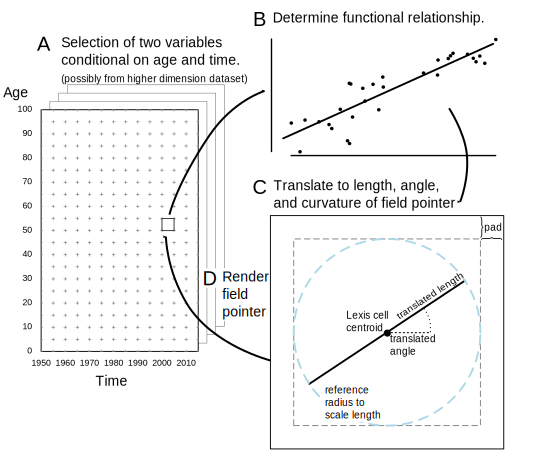
\includegraphics[scale=.8]{Figures/ExplainerDiagram.pdf}
  \caption{A diagram depicting the translation of functional relationships in data conditioned on age and time to visual encoding on a Lexis field. \textbf{A}: Condition data selection on age and time. \textbf{B}: model the functional relationship in data subset. \textbf{C}: Translate the model to field elements, `pointers', using angle, and possibly also length, curvature, thickness, etc to encode model qualities. \textbf{D}: Populate the Lexis plane with field pointers to create a Lexis field.}
  \label{fig:explain}
\end{figure}

\section{Application}
We select all HMD data available for females after 1950. For each lifetable we calculate two additional columns: the standard deviation of remaining lifespan $sd(x)$, and the coefficient of variation of remaining lifespan $CV(x)$. Each Lexis field element is based on the relationship between $sd(x)$ and remaining life expectancy $e(x)$ in 1$\times$5 Lexis cells\footnote{Data points included in regressions are single ages evenly divisible by five for each of the five years included in a Lexis reference cell.}, as summarized by bivariate linear regression over the data points in each cell. The regression results used for each Lexis cell in resulting Lexis fields are identical, but the translation of regressions to field pointers varies between designs. We offer four examples of Lexis field designs, displayed in Fig.~\ref{fig:figFields}, each rendered on 5$\times$5 Lexis subplots.

The first of these, Fig.~\ref{fig:sfig1}, is a bare-bones Lexis field that serves to illustrate the underlying concept. This display renders each regression slope as a line segment of equal length (4 ``years'' long) and centered on each Lexis cell. The slope of each pointer is rendered identical to regression slopes, which may be justified in this case, since Lexis cells fix a 1:1 year aspect ratio, while $e(x)$ and $sd(x)$ are also in year units. This is the truest and most literal depiction of how these regression slopes vary over age and time among HMD females, and nothing more. From this figure we can see, for example, that there is some age where the relationship turns from negative to positive, which increased slightly over time. Slopes dampened in younger ages around the 1980s, but have since increased (except infants).

The second version, Fig.~\ref{fig:sfig2}, also renders slopes on a unity aspect ratio, but lengths are proportional to the Pearson' correlation coefficient's $r$. Other measures of model fit could be used to similar effect to scale some characteristic of the field pointers. For example, Fig.~\ref{fig:sfig3} renders slopes multiplied by two, with pointer lengths scaled proportional to the between-population interquartile range of the $e(x)$ and $sd(x)$ values used in regressions\footnote{Specifically, pointer length is proportional to the central spread of the relationship between $e(x)$ and $sd(x)$, approximated as $\sqrt{IQR(e(x))^2 + IQR(sd(x))^2}$}, and line weight and grayscale ``proportional'' to the $r^2$ of the regression fit. Segment lengths are therefore indicative of the spread in the data, while higher Pearson's $r$ results in more contrast in the field. 

The final example, Fig.~\ref{fig:sfig4} is a true Lexis map. The base of the map is a filled contour plot of the mean (over HMD populations) coefficient of variation of the conditional remaining distribution $CV(x)$ in each single age and year. This map is redundantly coded with a sequential color palette and labelled contours, which liberates the surface from an explicit color legend. The same field from Fig.~\ref{fig:sfig3} is layered atop the CV surface, achieving a true layered map. In principle, one could represent variation in the slope of some other regression over age and time as a contour plot, with the present field atop, thereby layering comparable information. However, the present example serves to illustrate layering with the field.

% plain latex appears to work? would rather produce plots in chunk,
% but can't figure out how to do 2x2 panel of it.
\begin{figure}
\begin{subfigure}{.48\textwidth}
\captionsetup{width=.8\linewidth}
  \centering
  \includegraphics[scale=.38]{Figures/FigApp1.pdf}
  \caption{Lexis field: $sd(x)$ by $e(x)$ linear fits, with slopes drawn directly. Pointer lengths are all equal.}
  \label{fig:sfig1}
\end{subfigure}%
\begin{subfigure}{.48\textwidth}
\captionsetup{width=.8\linewidth}
  \centering
  \includegraphics[scale=.38]{Figures/FigApp2.pdf}
  \caption{Lexis field: $sd(x)$ by $e(x)$ linear fits, with slopes drawn directly. Pointer length is proportional to the Pearson's $r$.}
  \label{fig:sfig2}
\end{subfigure}
\begin{subfigure}{.48\textwidth}
\captionsetup{width=.8\linewidth}
  \centering
  \includegraphics[scale=.38]{Figures/FigApp3.pdf}
  \caption{Lexis field: $sd(x)$ by $e(x)$ linear fits, with slopes exaggerated by 2. Pointer length is proportional to the diagonal of the IQR box around $sd(x)$ and $e(x)$, while grayscale and segment width are proportional to Pearson's $r$.}
  \label{fig:sfig3}
\end{subfigure}%
\begin{subfigure}{.48\textwidth}
\captionsetup{width=.8\linewidth}
  \centering
  \includegraphics[scale=.38]{Figures/FigApp4.pdf}
  \caption{A Lexis map: Lexis surface of mean CV as a filled contour plot plus a Lexis field of $sd(x)$ by $e(x)$ linear fits, slopes exaggerated by 2. Pointer length is proportional to the diagonal of the IQR box around $sd(x)$ and $e(x)$, while grayscale and segment width are proportional to Pearson's $r$.}
  \label{fig:sfig4}
\end{subfigure}
\caption{Four versions of Lexis fields displaying the linear
relationship between the standard deviation and mean of remaining
lifespan, females (HMD).}
\label{fig:figFields}
\end{figure}

\section{Discussion}
We suggest the use of vector fields on the Lexis surface, introducing the notion of a Lexis field, which is a standard vector field on a regular Lexis grid over age and time. We demonstrate some of the designer degrees of freedom in translating data into the elements of a Lexis field, as well as an instance of Lexis map layering. These examples serve to illustrate the construction of Lexis fields, but do not pretend to be ``best practice'' Lexis surfaces in terms of visual design or legibility. It is our sense that the patterns revealed in Figures~\ref{fig:sfig1}-\ref{fig:sfig3} are accessible to the viewer and lend themselves to substantive interpretation. This visual instrument indeed arose in practice in an attempt to investigate the apparently mechanical relationship between lifespan variation and average length of life with a macro view. Fig.~\ref{fig:sfig4} simply serves to illustrate that Lexis fields can be layered with traditional Lexis surfaces that are color coded, increasing the information and pattern density on the Lexis plane with little drawback in terms of legibility. 

Although patterns in data may be much more complex than can be expressed with linear models, these simple model fits can be thought of as regular samples from the complex space implied by data, such that the pattern revealed on the Lexis field is still revealing. On the other hand a field may be derived from a single underlying pattern rather than a series of regressions on different populations or variables. For example, \citet{shang2018visualizing} recommends the use of derivative phase diagrams to represent the rate of change of the hypothetical lifecourse implied by period fertility curves. This construct could be translated to a Lexis field in a straightforward way, with pointers mapping to the notions of acceleration and velocity. Certainly variants of vector fields could be used to intuitively render other demographic phenomena and components of demographic change, and these do not need to adhere to the Lexis grid. Indeed, we suggest the use of fields based on demographic relationships in spatial settings.

\section{Conclusions}
We describe the construction and use of vector fields on the Lexis plane. We argue that this technique can increase the information density and scope displayed on the Lexis surface. We also argue that the visual encoding of fields is easily made compatible with Lexis surfaces rendered as filled contour plots, which lends itself to map layering. We suggest alternative visual encodings and uses. In sum, displaying a larger variety of demographic quantities on the Lexis plane and increasing the information density on the Lexis plane using layering techniques such as fields should broaden the scope of demographic exploration and sharpen the instruments of demographic pattern detection.

\section{Reproducibility}
Code used to produce the experimental visualizations here is available in a public repository: 

%\url{https://github.com/timriffe/MacroShape/DR}
\blackout{\url{https://github.com/timriffe/MacroShape}}

\section{Acknowledgements}
%We wish to thank \blackout{Alyson van Raalte} for helpful comments received that improved this manuscript.
We wish to thank Alyson van Raalte for helpful comments received that improved this manuscript.

\FloatBarrier
\singlespacing
\bibliographystyle{DemRes}
  \bibliography{references} 

\end{document}
